\section{Auswertung}
\label{sec:Auswertung}

\subsection{Aufnahme der Zählrohr-Charakteristik}
In Tabelle \eqref{tab:Char} ist die Zähltrate $N$ in Abhängigkeit von der Spannung $U$ aufgezeigt. Im folgenden wird allerdings nur mit den nicht ausgegrauten Werten gerechnet, da nur diese zu dem Plateau der Charakteristik gehören. Das Plateau liegt wie in Abbildung \eqref{fig:Char1} zu sehen ist, zwischen 350\,V und 650\,V. Mit Hilfe einer Ausgleichsrechnung wird die Funktion des Plateaus zu
\begin{equation*}
  y = (\num{0.09 +- 0.02}) \cdot x + (\num{500 +- 10})
\end{equation*}
bestimmt. Für die Steigung in \% pro 100\,V ergibt sich
\begin{equation*}
  m = \frac{a\cdot100}{N(500\,V)} = \frac{(\num{0.09 +- 0.02})\cdot100}{545} = (\num{0.017 +- 0.004})\% \ .
\end{equation*}

\begin{table}[H]
  \centering
  \begin{tabular}{c|c|c|c}
    \hline
    $U$ / V & n / 10\,s & N / $\frac{1}{\text{s}}$ & $\frac{\sqrt{n}}{n}$ \\
    \hline
    \rowcolor{lightgray} 310 & 4634 & & \\
    \rowcolor{lightgray} 315 & 5059 & & \\
    \rowcolor{lightgray} 325 & 5223 & & \\
    \hline
    \hline
    350 & 5437 & $\num{544 +- 7}$ & 0.01 \\
    375 & 5384 & $\num{538 +- 7}$ & 0.01 \\
    400 & 5368 & $\num{537 +- 7}$ & 0.01 \\
    450 & 5405 & $\num{541 +- 7}$ & 0.01 \\
    500 & 5447 & $\num{545 +- 7}$ & 0.01 \\
    550 & 5552 & $\num{555 +- 7}$ & 0.01 \\
    600 & 5485 & $\num{549 +- 7}$ & 0.01 \\
    625 & 5598 & $\num{560 +- 7}$ & 0.01 \\
    650 & 5745 & $\num{575 +- 8}$ & 0.01 \\
    \hline
    \hline
    \rowcolor{lightgray} 675 & 6028 & & \\
    \rowcolor{lightgray} 700 & 6264 & & \\
    \rowcolor{lightgray} 705 & 6443 & & \\
    \hline
  \end{tabular}
  \caption{Messwerte für die Charakteristik des Zählrohrs.}
  \label{tab:Char}
\end{table}

\begin{figure}[H]
  \centering
  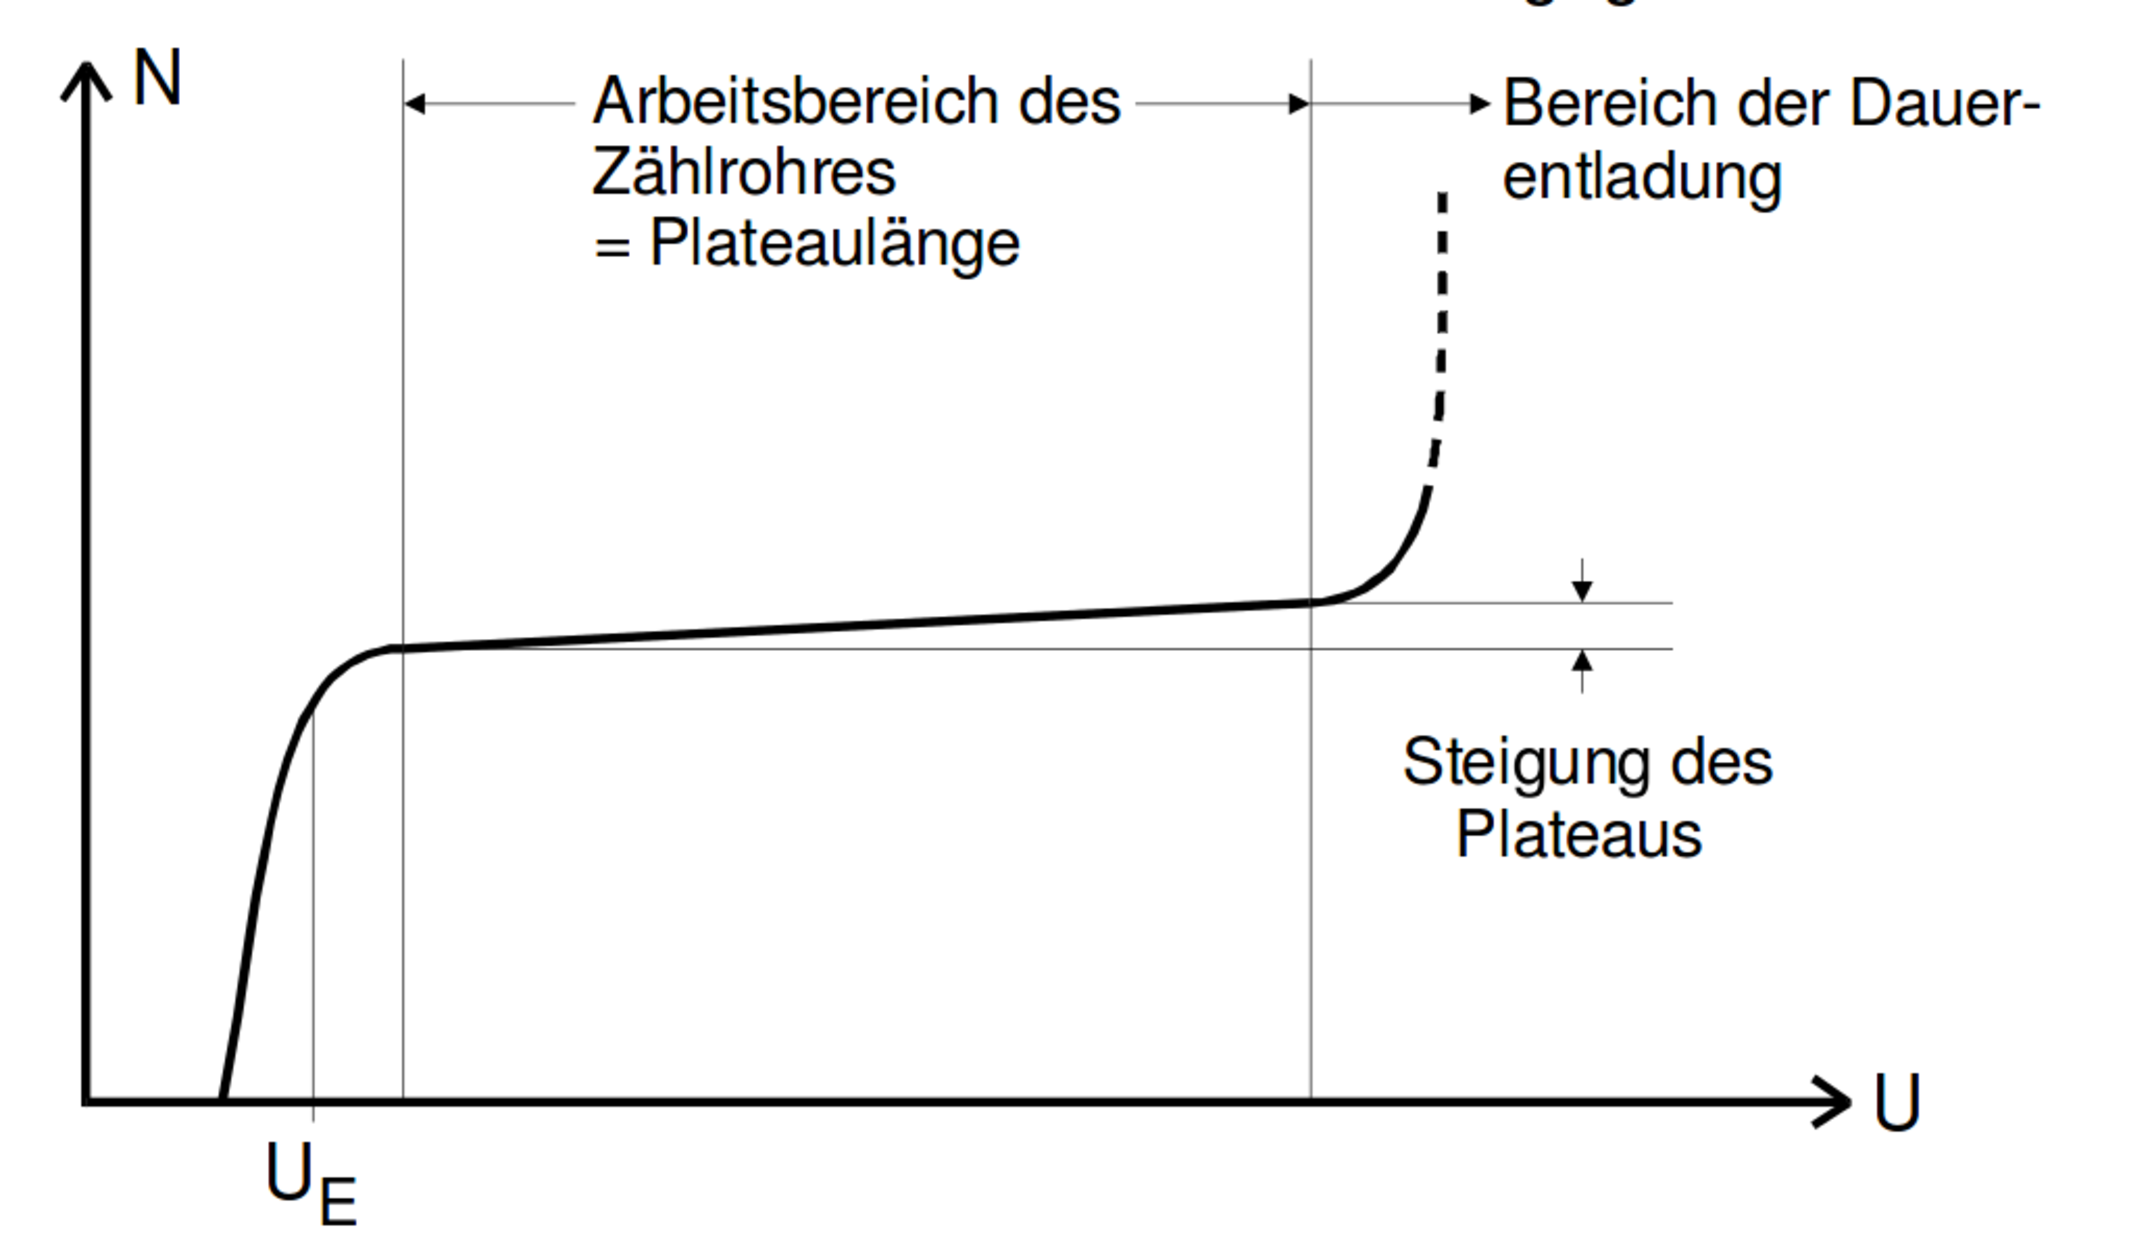
\includegraphics[height=10cm]{build/Plateau.pdf}
  \caption{Charakteristik des Zählrohres.}
  \label{fig:Char1}
\end{figure}


\subsection{Sichtbarmachung von den Nachentladungen}
Zu Beginn dieses Versuchteils wird die Strahlintensität soweit abgesenkt das nur ein Primärmaximum bei 350\,V auf dem Oszillographen zu sehen ist. Dann wird bei einer Ablenkgeschwindigkeit von 50 $\mu$s/cm der Abstand zwischen Primär- und Nachladeimpuls geschätzt. Dieser beträgt für 350\,V ($\num{220 +- 50}$)\,$\mu$s und für 700\,V ($\num{215 +- 50}$)\,$\mu$s.


\subsection{Bestimmung der Totzeit}
Die Totzeit wird auf zwei Arten gemessen. \\
Bei der ersten Methode wird die Totzeit gemäß der Abbildung \eqref{fig:} für 350\,V und 700\,V abgelesen.
\begin{align*}
  T_\text{350\,V} = (\num{50 +- 2})\,\mu\text{s} \\
  T_\text{700\,V} = (\num{70 +- 2})\,\mu\text{s} \\
\end{align*}
Der Mittelwert daraus beträgt
\begin{align*}
  T = (\num{60 +- 1})\,\mu\text{s}
\end{align*}
Die Messwerte für die zweite Messung sind im folgenden aufgelistet:
\begin{align*}
  N_1 = (\num{425 +- 7}) \\
  N_2 = (\num{336 +- 6}) \\
  N_{1+2} = (\num{704 +- 8}) \\
\end{align*}
Daraus lässt sich mit
\begin{align*}
  T = \frac{N_1 + N_2 - N_{1+2}}{2\,N_1\,N_2} \ ,
\end{align*}
eine Totzeit von
\begin{align*}
  T = (\num{0.20 +- 0.04})\,\text{ms}
\end{align*}
berechnen.

























\subsection{}
